\chapter{Case Study: S\~ao Paulo Simulation}
\label{cap:sao_paulo}

This chapter presents the simulation of the city of S\~ao Paulo as a use case of InterSCSimulator. Also, we validated and verified the models described in Chapter \ref{cap:interscsimulator} using this scenario. The simulation validation and verification are critical to demonstrating that the models are working and producing useful results. This simulation is also the basis for the scalability analyzes presented in Chapter \ref{cap:avaliacao}.

\section{Input Data}

We based our simulation in real data collected from different sources. The databases considered in this simulation are:

\begin{itemize}

\item Origin-Destination (OD) Matrix derived from a survey conducted by the city subway company for the year 2012\footnote{Origin-Destination Survey - \url{http://goo.gl/Te2SX7}}

\item Map of the city based on OpenStreetMap \footnote{OpenStreetMap - https://www.openstreetmap.org}

\item Buses lines and stops of the city provided by the Municipal Transportation Secretary

\item Subway network of the city provided by the Metr\^o Company

\end{itemize}

\subsection{Origin-Destination Survey}

The OD survey of the city has more than 60 thousand registers. Each register contains information about travel of one person from an origin to a destination which are different places in the city such as houses, workplaces, and schools. Besides the origin and destination, there are other valuable data about the travels such as the start time, expected arrival time, and transportation mode. The survey has information about bus, cars, rides, bicycle, suburban trains, and subway travels.

Other fundamental information to the simulator is an extrapolation factor which estimates the number of people that make similar trips to the person of the OD register. We use this data to simulate the entire city population randomly positioning the people of the extrapolation factor close to the original position of the OD. With this information, there are more than 20 million travels and 11 million people in the OD, what is very close to the entire population of the city of S\~ao Paulo. 

Figure \ref{fig:travel_count_mode} presents the number of travels in the OD survey. There are 5.058.002 million travels by car, 4.029.546 million travels by buses, 6.287.487 million travels on foot, and 3.030.809 million travels by subway or suburban train. The figure shows that most of the city population makes their trips walking or using public transportation, especially buses. However, there are also a huge number of cars in the city streets. The OD survey has data about other transportation modes such as cars passengers, bicycles, taxis, and school buses. We did not consider these modes because some of them do not impact the traffic such as car passengers or we do not have real data to make useful simulation such as bicycles, taxis, and school buses.

\begin{figure}[!htb]
\centering
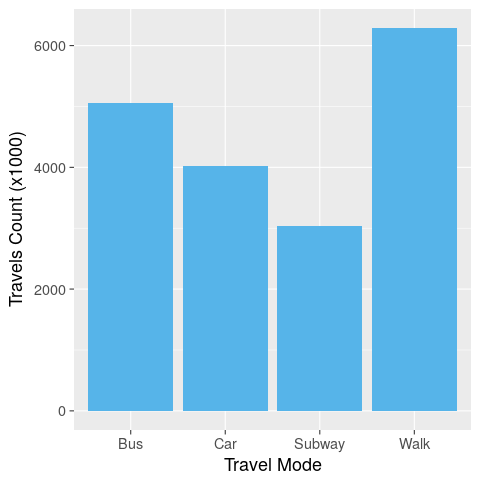
\includegraphics[width=0.6\textwidth]{figuras/chap-sp/travel_count.png}
\caption{Total Number of Trips by Transportation Mode}
\label{fig:travel_count_mode}
\end{figure}

Another essential information to the simulation is the time when each person starts his travel. Figure \ref{fig:travel_count_mode_and_hour} presents the travels start time grouped by the start time using 1-hour intervals. This chart shows that there is a considerable variation in the number of travels during the day. Most of the travels are during the peak hours (from 6 to 9 am and from 5 to 8 pm) and at the lunchtime. However, most of the travels during lunch time are on foot or by subway and are small travels. Probably they are performed by people going from their work to restaurants or home to lunch.

\begin{figure}[!htb]
\centering
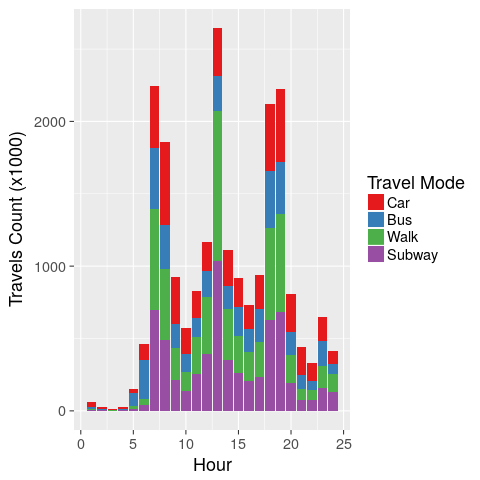
\includegraphics[width=0.6\textwidth]{figuras/chap-sp/mode.png}
\caption{Number of Trips by Transportation Mode and by Hour}
\label{fig:travel_count_mode_and_hour}
\end{figure}

Another relevant information is that the OD survey has only the primary transportation mode of the commuters. Hence, it is possible that many people use more than one transportation mode during one travel. For example, in S\~ao Paulo it is common to have buses from a neighborhood that go to subway stations, where most of the people take the subway to arrive at the downtown. Finally, the OD has the expected travel time of the commuters. We used this information to verify if the used mobility models are generating reasonable results.

A problem with the OD survey is that it is updated every five years. Of course, there are many changes in the city mobility in this interval. However, even with this problem, the OD survey is the most representative data about S\~ao Paulo mobility patterns.

\subsection{City Map}

We used the OpenStreetMap to generate the graph of the city. This graph has approximately 50 thousand nodes and 120 thousand links and covers most of the streets and roads of S\~ao Paulo and some parts of its metropolitan area. In the graph, the links represent stretches of the streets and the nodes the intersections. All the nodes in the graph have a unique id and their latitude/longitude. The links have the start and end node, the maximum speed, the length, the type, and the capacity of the street. With this graph, we can implement all the models described in Section \ref{sub:modelo}.

\subsection{Bus Lines and Stops}

To simulate the buses lines and stops of S\~ao Paulo, we used the data from the city transportation secretariat (SPTrans). They provided a spreadsheet with all the lines of the city with information about them such as the code, the stops, the start time, and the average interval of the buses along the day.

There are 2,347 lines in the city, and they have different characteristics. For example, some lines run only on weekends and lines that work just for a few hours, mainly in the peak hour. The numbers of stops can also vary a lot from line to line, on average each bus makes 43 stops in its route. However, there are buses with just four stops and others with 144 stops. Regarding the stops, S\~ao Paulo has 19,144 bus stops. As about the buses, there is a significant variance about the stops in the city. In average, five buses pass through each stop in the city. However, there are stops with just 1 line and others with 62 lines.

\subsection{Subway and Suburban Trains Network}

To simulate the subway and train system of S\~ao Paulo we created a digraph using the data about the lines of the city. Although different companies manage the train and the subway system (CPTM and Metrô), both systems are integrated and have the same cost to the users. The subway system has six lines, 79 stations, and an extension of almost 90 kilometers. The train network has seven lines, 90 stations, and an extension of more than 270 kilometers. Together, the two systems have more than 4 million users per day. 

\section{Simulation Execution}

Based on the data described in the last section, we created all the input files of InterSCSimulator and simulated an entire day in the city. The simulation was executed in a machine on the Google Cloud Environment with a memory of 160 GB and 16 cores. The simulation took approximately 7 hours to execute and at the peak used 138 GB of memory. The output file generated by the simulation has more than 17 million travels and occupy 2 GB of the disk.

\section{Validation and Verification}

According to Sargent \cite{sargent2013verification} to confirm if a simulator is generating useful results, it is essential to validate and verify the simulator output. The validation consists in analyzing if the models and data structures are working and generating the expected outputs. The verification compares the simulation results with the real system and the analyzed variables must be equal or very close in both cases. To validate the models we made several analyzes in the results of the simulator and to verify the simulation models we compared the real travel time of the OD survey with the simulated travel time. 

\subsection{Validation}

The output of the simulator is a mobility trace with all the events that occurred in the simulation. To analyze the travel times, we filtered just the arrival events which occur when a commuter arrives at his destination. In this event, we save the total travel time and distance. With this data, we made analyzes about the mobility patterns in the city. For example, to show the concentration of people and vehicles, we generated a heat map with the agents in S\~ao Paulo downtown. Figure \ref{fig:heat_map} shows the people and vehicles in the morning peak hour, between 8 and 8:10. The Figure presents a significant concentration of vehicles in important avenues of the city such as 23 de Maio and Radial Leste which are known for their great congestion.

\begin{figure}[!htb]
\centering
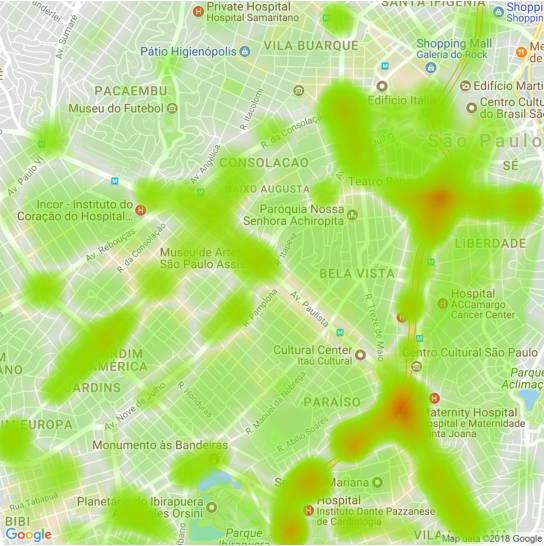
\includegraphics[width=0.8\textwidth]{figuras/chap-sp/mapa_calor.pdf}
\caption{Heat map of the simulated travels}
\label{fig:heat_map}
\end{figure}

\subsubsection{Vehicles Travels}

Figure \ref{fig:travel_time2} shows the analyzes to car travels with the mean travel time, distance, and speed of the vehicles depending on the arrival time of their arrival time. The last chart shows the total number of vehicles that finished a trip for each hour of the simulation.

\begin{figure}[!htb]
\centering
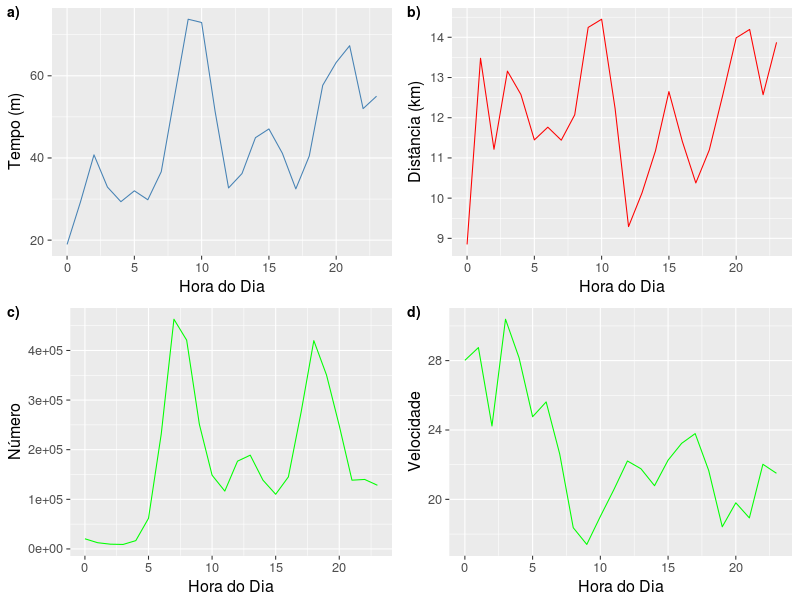
\includegraphics[width=1\textwidth]{figuras/chap-sp/time_distance_car.png}
\caption{Analyzes of the car travels}
\label{fig:travel_time2}
\end{figure}

The charts show that on average the travels are much slower in the peak hours than during the rest of the day. It is mainly due to the decrease in the average speed of the vehicles caused by the massive amount of vehicles that are moving in the city. It is also possible to verify that the distance is not very important in the travel time, the average distance of the travels varies from 10 km to 14 km during the day.

Figure \ref{fig:scatter_car} presents the correlation of time, distance, the hour of the day, and the speed of car travels. The Figure shows that some variables are very correlated such as time and distance and speed and time. Otherwise, there is no visible correlation between the distance and hour of the day and distance and speed.

\begin{figure}[!htb]
\centering
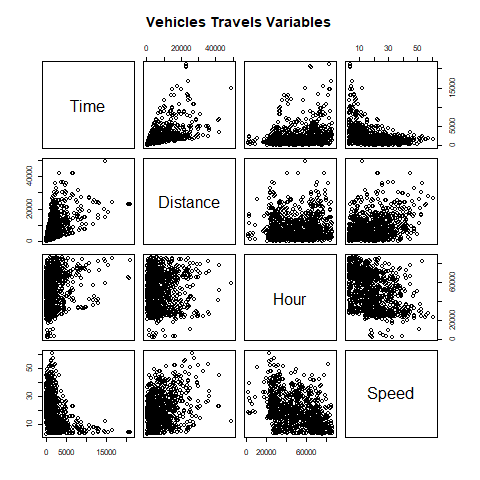
\includegraphics[width=0.8\textwidth]{figuras/chap-sp/scatter_car.png}
\caption{Correlation among Car travels variables}
\label{fig:scatter_car}
\end{figure}

\subsubsection{Subway Travels}

Figure \ref{fig:scatter_subway} presents the correlation of time, the hour of the day, and the number of stations on subway travels. As the chart shows, the number of stations define the inferior limit of the travel time. However, a significant part of the subway travel uses another transportation mode such as buses or walking. The chart also shows that there is a higher number of travels during the peaks hours, in the morning, at the lunchtime, and at the final of the afternoon.

Also, the chart shows that are a small number of travels in the very beginning of the day because the subway system of S\~ao Paulo works until approximately 00:30. The last train of almost all lines depart at midnight, and each station closes after this train leaves. The system opens at 04:40 every day. 

\begin{figure}[!htb]
\centering
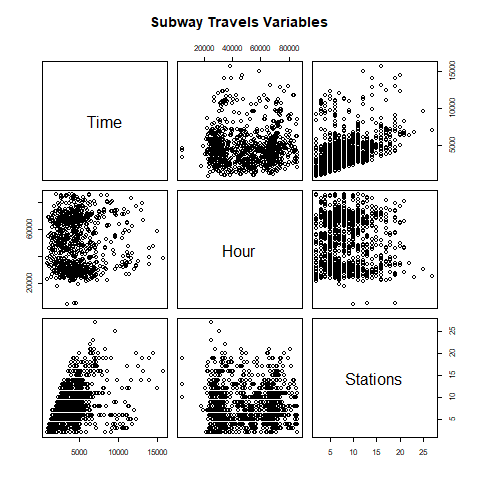
\includegraphics[width=0.8\textwidth]{figuras/chap-sp/scatter_subway.png}
\caption{Correlation among Subway travels variables}
\label{fig:scatter_subway}
\end{figure}

A limitation of our work is that in the peak hours it is probably that a user will take some time waiting for a train in a station, it occurs because the trains already arrive full or there is a massive queue to enters the train. We do not model this time wasted to get the next train yet. However, it is possible to create a model that calculates the time to enter a train based on the number of people that is in the stations.

\subsubsection{Pedestrian Travels}

Figure \ref{fig:scatter_walk} presents the correlation of time, the hour of the day, and the distance of pedestrian travels. The Figure shows that there is a linear correlation between the time and distance variables, and there is no correlation between the hour and time and hour and distance. The chart also shows that the travels are evenly distributed during the day, except during the dawn.

\begin{figure}[!htb]
\centering
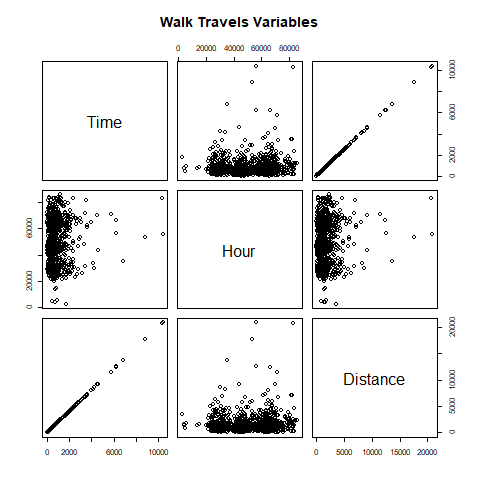
\includegraphics[width=0.8\textwidth]{figuras/chap-sp/scatter_walk.png}
\caption{Correlation among Pedestrian travels variables}
\label{fig:scatter_walk}
\end{figure}

Our pedestrian model is simple, but it is possible to extend it adding information about the pedestrian such as age and mobility difficulties. We did not find any model in the literature that use personal information to model the pedestrian speed, but the information is available in the origin-destination survey.

\subsubsection{Bus Travels}

The bus travels also suffer the impact of the traffic in the city. Figure \ref{fig:travel_time_bus} shows the mean travel time of the buses ad the total number of arrivals per hour.  In the first graph is possible to verify that the mean travel time of the buses in the peak hour are almost 15\% bigger than the other hours. Also, as showed in the second chart, during the peak hours the number of buses moving in the city is almost the double of the rest of the day.

\begin{figure}[!htb]
\centering
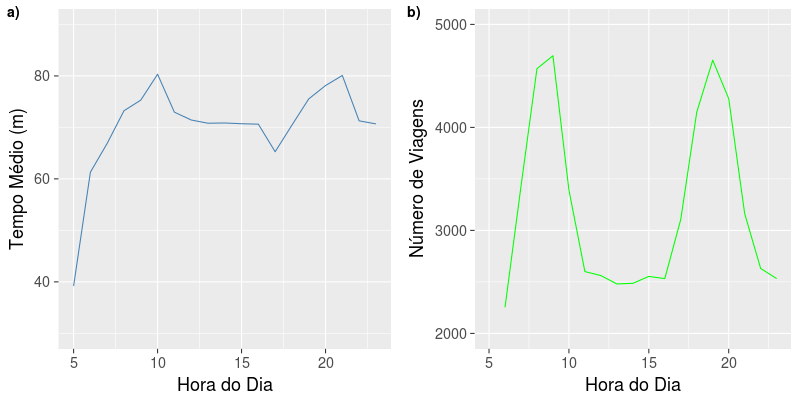
\includegraphics[width=1\textwidth]{figuras/chap-sp/time_distance_bus.png}
\caption{Analyzes of bus travels}
\label{fig:travel_time_bus}
\end{figure}

Regarding the people that travel by bus, Figure \ref{fig:scatter_bus} presents the correlation of time and the hour of the day. The chart shows that exists many long travels with more than 3 hours and the bigger trips are during the morning peak and in the night starting in the night peak.

\begin{figure}[!htb]
\centering
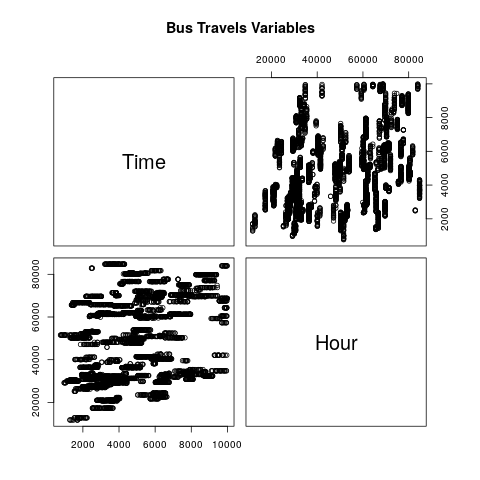
\includegraphics[width=0.8\textwidth]{figuras/chap-sp/scatter_bus.png}
\caption{Correlation among Bus travels variables}
\label{fig:scatter_bus}
\end{figure}

\subsection{Verification}

To verify the models, we compared the real travel time that is in the OD survey with the simulation travel time. This approach has some limitations, for example, most of the answers in the OD are rounded, because typically people approximate their travel time when answering the survey. Another problem is that the OD is from 2012 and we are using the mobility infrastructure of 2018. In the pedestrian and cars travels it will have a limited impact as the streets and roads did not change so much. However, the bus and subway travels are significantly affected by this problem because the city now has new subway lines, and the bus lines are modified continuously.

Figure \ref{fig:box_plot_real_simulated} presents the comparison of all travels. The chart shows that the travel time from simulated and real environments is between 300 and 6000 seconds. The median of the simulated travels are 1800 seconds and of the real travel are 1840 seconds, an error of only 2,5\%. This difference is caused mostly by the buses travels as we will show in the next figures.

\begin{figure}[!htb]
\centering
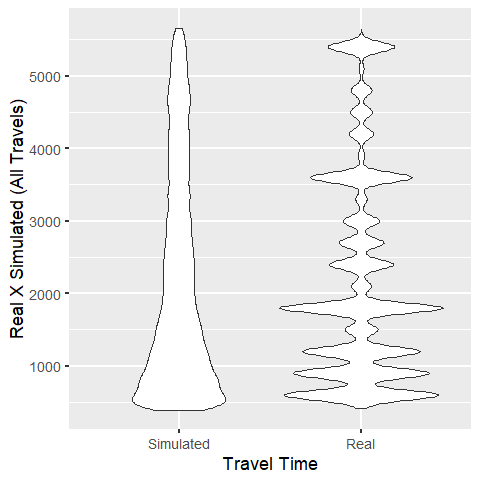
\includegraphics[width=0.5\textwidth]{figuras/chap-sp/total.png}
\caption{Travel time in real and simulated environments}
\label{fig:box_plot_real_simulated}
\end{figure}

Figure \ref{fig:box_plot_real_simulated_bus_subway} presents the comparison of cars and pedestrian travels. Regarding the cars travel, the chart shows that the travel time from simulated and real environments is between 300 and 5000 seconds. The median of the simulated travels is 1655 seconds and of the real travel are 1756 seconds, a difference of 6\%. This difference shows that the mesoscopic model used in the InterSCSimulator is reproducing well the city environment.

Regarding the pedestrian travels, the chart shows that the travel time from simulated and real environments is between 300 and 3000 seconds. The median of the simulated travels are 880 seconds and of the real travel are 868 seconds, a difference of 1\%. This difference shows that the model used in the InterSCSimulator is reproducing well the city environment, mainly because simulating a mesoscopic pedestrian behavior is very straightforward.

Figure \ref{fig:box_plot_real_simulated_bus_subway} presents the comparison of subway and bus travels. Regarding the subway travels, the chart shows that the travel time from simulated and real environments is between 300 and 7000 seconds. The median of the simulated travels are 4080 seconds and of the real travel are 3805 seconds, a difference of 7\%. The subway model is also simple to simulate, most of the difference in this model is caused by the buses that are used by some commuters to arrive at a subway station.

Regarding the bus travels, the chart shows that the travel time from simulated and real environments is between 1000 and 6000 seconds. The median of the simulated travels is 3585 seconds and of the real travel are 3240 seconds, an error of 11\%. This difference shows that the model used in the InterSCSimulator is not reproducing well the city environment. The cause of this difference is that the bus travels are much harder to reproduce for different reasons such as the schedule of the buses varies a lot in S\~ao Paulo, the city has more than 2000 lines, and it is necessary to analyze one by one to reproduce the exact itinerary of the buses. Finally, for commuters that use more than one bus line, it is hard to reproduce their exact itinerary.

A work based on the simulator developed in a Smart City course implemented a much better bus model to the simulator. However, we did not integrate this model with the original models of InterSCSimulator yet. We will present this model in Section \ref{sec:mobiity_model}.

\begin{figure}[!htb]
\centering
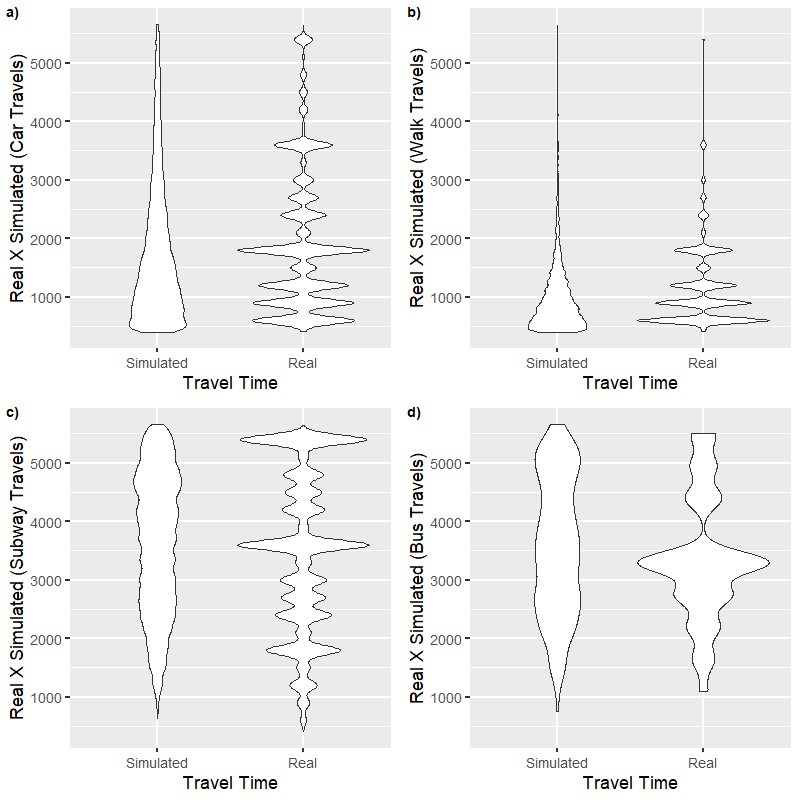
\includegraphics[width=1\textwidth]{figuras/chap-sp/total_modes.png}
\caption{Car, Pedestrian, Subway and Bus Travel time in real and simulated environments}
\label{fig:box_plot_real_simulated_bus_subway}
\end{figure}
